\documentclass [listof=totoc,bibliography=totoc,english,a4paper,titlepage] {scrartcl}

\usepackage[english]{babel}
\usepackage{setspace}
\usepackage[paper=a4paper]{geometry}
\usepackage[utf8]{inputenc}
\usepackage{amsmath}
\usepackage{dsfont}
\usepackage{graphicx}
\usepackage{textcomp}
\usepackage{subfigure}
\usepackage{esvect}
\usepackage{pstricks}
\usepackage{floatflt}
\usepackage{SIunits}
\usepackage{amsopn}
\usepackage[percent]{overpic}
\usepackage{newclude}

\setlength{\parskip}{6pt}
\setlength{\parindent}{0pt}

\onehalfspacing

\renewcommand{\thefigure}{\arabic{section}.\arabic{figure}}
\makeatletter \@addtoreset{figure}{section} \makeatother
\renewcommand{\thetable}{\arabic{section}.\arabic{table}}
\makeatletter \@addtoreset{table}{section} \makeatother
\renewcommand{\theequation}{\arabic{section}.\arabic{equation}}
\makeatletter \@addtoreset{equation}{section} \makeatother

\let\oldbibitem=\bibitem
\renewcommand{\bibitem}{%
\filbreak
\oldbibitem
}

\newenvironment{changemargin}[2]{%
  \begin{list}{}{%
    \setlength{\topsep}{0pt}%
    \setlength{\leftmargin}{#1}%
    \setlength{\rightmargin}{#2}%
    \setlength{\listparindent}{\parindent}%
    \setlength{\itemindent}{\parindent}%
    \setlength{\parsep}{\parskip}%
  }%
  \item[]}{\end{list}}


\newenvironment{mylisting}
{\begin{list}{}{\setlength{\leftmargin}{1em}}\item\scriptsize\bfseries}
{\end{list}}

\DeclareMathOperator{\grad}{grad}

\makeatletter
\let\divsymb\div              % make \IEEEendproof do same as \endproof
\let\div\@undefined                  % undefine \endproof
\makeatother

\DeclareMathOperator{\div}{div}

\begin{document}

%
%% Titelblatt
%%


\thispagestyle{empty} %% ohne Kopf- und Fusszeile, Seitennummer etc.

%% eigene Umgebung schaffen -> minipage
\begin{titlepage}     %% Anfang Sichtfenster

	\sffamily
	\begin{center}
		\vspace{1cm}
		
		\large{\textbf{Rheinisch-Westfälische Technische Hochschule Aachen\\Institut für Bildsame Formgebung}}
		
		\vspace{20mm}
				
		\Large{\textbf{Title bla blubb \\}}
		%\vspace{-0.35cm}
		\Large{\textbf{blubb bla}}
		
		\vspace{2cm}
		

		
		\LARGE{\textbf{Hauptseminar}} \\
		
		\vspace{1.5cm}
		
		\large{Paul Hibbe, B.Sc. \\ Matthias Nick, B.Sc.}\\
		
		\vspace{3cm}
		\end{center}
		
	%\large{Thema:\hspace{0.5cm}	Vergleich unterschiedlicher Dehnungsmessmethoden im quasistatischen Zugversuch\\ \hspace{2.0cm}}

	
\begin{center}
\large{Durchgeführt in der Abteilung Werkstoffmodellierung \\ im WS 2013/14}
\end{center}

\vspace{3cm}
\begin{tabbing}
\hspace*{3cm}\=\hspace{2cm}\=\kill
Betreuer: \>Univ. Prof. Dr.-Ing. Gerhard Hirt\\
          \>Dipl.-Ing. Thomas Henke\\
          \>Stephan Hojda, M.Sc.
\end{tabbing}
\end{titlepage} %% Ende Sichtfenster

\setcounter{tocdepth}{2}
\tableofcontents

\pagebreak

\section{Einleitung}

In der Fertigung von Prototypen und Kleinserien ist die Anwendung traditioneller Blechumformverfahren wie des Tiefziehens oder des Streckziehens aufgrund der Notwendigkeit von hochfesten Werkzeugen und Maschinen, die hohe Kräfte aufbringen können, sowohl kosten- als auch zeitintensiv. Ein Prozess, der diese Beschränkungen umgeht, ist die inkrementelle Blechumformung (IBU), welche mit einem universellen Werkzeug, das Blech inkrementell umformt. Für die IBU ergeben sich jedoch einige Prozessgrenzen. Neben der langen Dauer des Prozesses und seiner schlechten Abbildbarkeit in Simulationen sind dies insbesondere die Neigung zu Ausdünnung, Einschnürung und schließlich Riss des Blechs bei hohen Wandwinkeln sowie die schlechte Geometriegenauigkeit. \cite{dissbambach,dissames}\par

Das Problem der Geometriegenauigkeit zeigt sich besonders bei schwerumformbaren Werkstoffen wie dem in der Luftfahrt oft verwendeten TiAl6V4. Dieses besitzt neben einem niedrigen Elastizitätsmodul auch eine hohe Fließgrenze, so dass ein großer elastischer Anteil an der Formänderung besteht. Dies wiederum führt zur Rückfederung des Werkstücks nach dem Umformen. Weiterhin ist das Umformvermögen von TiAl6V4 bei Raumtemperatur nur gering. Zur Überwindung dieser Prozessgrenzen wurden bereits Versuche unternommen, die Fließspannung des umzuformenden Blech durch Erwärmung zu senken. Neben der Erwärmung des gesamten Bleches während des Prozesses ist es möglich, den Werkstoff gezielt in der Umformzone zu erwärmen. Dies kann konduktiv oder mit Laserstrahlung erfolgen. \cite{hybridisf,diplbailly}\par

Zur laserunterstützten inkrementellen Blechumformung ist bereits eine Optik entwickelt worden, die es ermöglicht, den Laserbrennfleck um das Umformwerkzeug herum zu bewegen. Ebenfalls existiert bereits ein Programm, welches auf Basis eines bestehenden NC-Pfads zu einem IBU-Prozess die notwendigen Bewegungen des Laserbrennflecks bestimmt \cite{laseraisfti}. Es ist jedoch aus thermischen und geometrischen Gründen nicht sinnvoll, den Laser dauerhaft mit der gleichen Ausgangsleistung zu betreiben. Daher ist das Thema dieser Arbeit eine Vorausberechnung der benötigten Laserleistung unter Berücksichtigung der tatsächlichen Geschwindigkeit des Laserbrennfelcks und von Wärmeleitungs- und Wärmeverlustphänomenen sowie eine theoretische Validierung des dazu entwickelten Algorithmus und das Erstellen eines Konzepts für die Einbindung in das bestehende CAX-Umfeld.
\section{Fundamentals}

\subsection{Open-die forging}
The incremental and flexible nature of open-die forging makes it suitable primarily to the manufacturing of small lot sizes or for the forming of parts that cannot be produced by other processes due to power and force limitations of these processes. Its primary use is in the preparation of cast ingots for further machining. By open-die forging, cavities from the casting process can be rectified and the needed material properties can be reached.\cite{forgcomp}

\subsection{Finite element method}
The finite element method is a method to model, beside others, continuum mechanics of solid work pieces. The work piece is separated into discrete parts, called elements, which are themselves geometrically defined by nodes. While these nodes hold coordinates as information, the elements hold temperatures, stresses etc. Using material properties such as flow curves, friction, thermal conductivity and emissivity, the system's reaction to thermal and mechanical external loads can be calculated.

Due to the non-linear nature of the resulting equation system, only very simple models can be calculated analytically while most must be approximated numerically. Besides matters of usability, the numerical approach is the most important difference between available software packages. These are spread across a wide spectrum from academic systems with large freedom for the user to easy-to-use specialized tools for certain uses.

\section{Model process}
\label{sec:model_process}
This work deals with modeling of an open die forging process with multiple passes. The material used is a common stainless steel. The process parameters are orientated on a plan for forging a block with four passes given by the forging simulation software ForgeBase. Important process parameters, besides the flow curves, are for example the material data, the height reduction during every pass, the movement of the die, meaning the kinematics, the process temperature, etc. The detailed process conditions are discussed in the following chapters.\par

\subsection{Material data}
The material used is a 1.4301 (X5CrNiMo18-10) stainless steel. It is an austenitic steel which contains high quantities of the alloying elements chrome and nickel \ref{table:chemicalcomposition}. Therefore it is non-corrosive, acid- and heat-resistant. The field of application is widely spread and reaches from the automotive industry up to the chemical industry \cite{1.4301}.\par

The chemical composition (in weight-\%) of the material is as follows \cite{metallograf.de}:
\begin{table}[htbp]%[width=1.0\textwidth]
 \footnotesize
 \centering
 \caption{Chemical composition of 1.4301}
 \begin{tabular}{|c|c|c|c|c|c|c|c|}
 \hline
 C[\%]&Cr[\%]&Ni[\%]&Si[\%]&Mn[\%]&P[\%]&S[\%]&N[\%]\\\hline
 max 0,07&17,00-19,50&8,00-10,50&max 1,00&max. 2,00&max 0,045&max 0,03&max 0,11\\\hline
 \end{tabular}
 \label{table:chemicalcomposition}
\end{table}\par

For the input in a simulation model the thermal material data is crucial, containing are the temperature depending thermal conductivity, the spec. heat capacity and the Young´s modul, see figure \ref{img:thermalconductivity}, \ref{img:heatcapacity}, \ref{img:youngsmodul}. 

\begin{figure}[htbp]
 \centering
 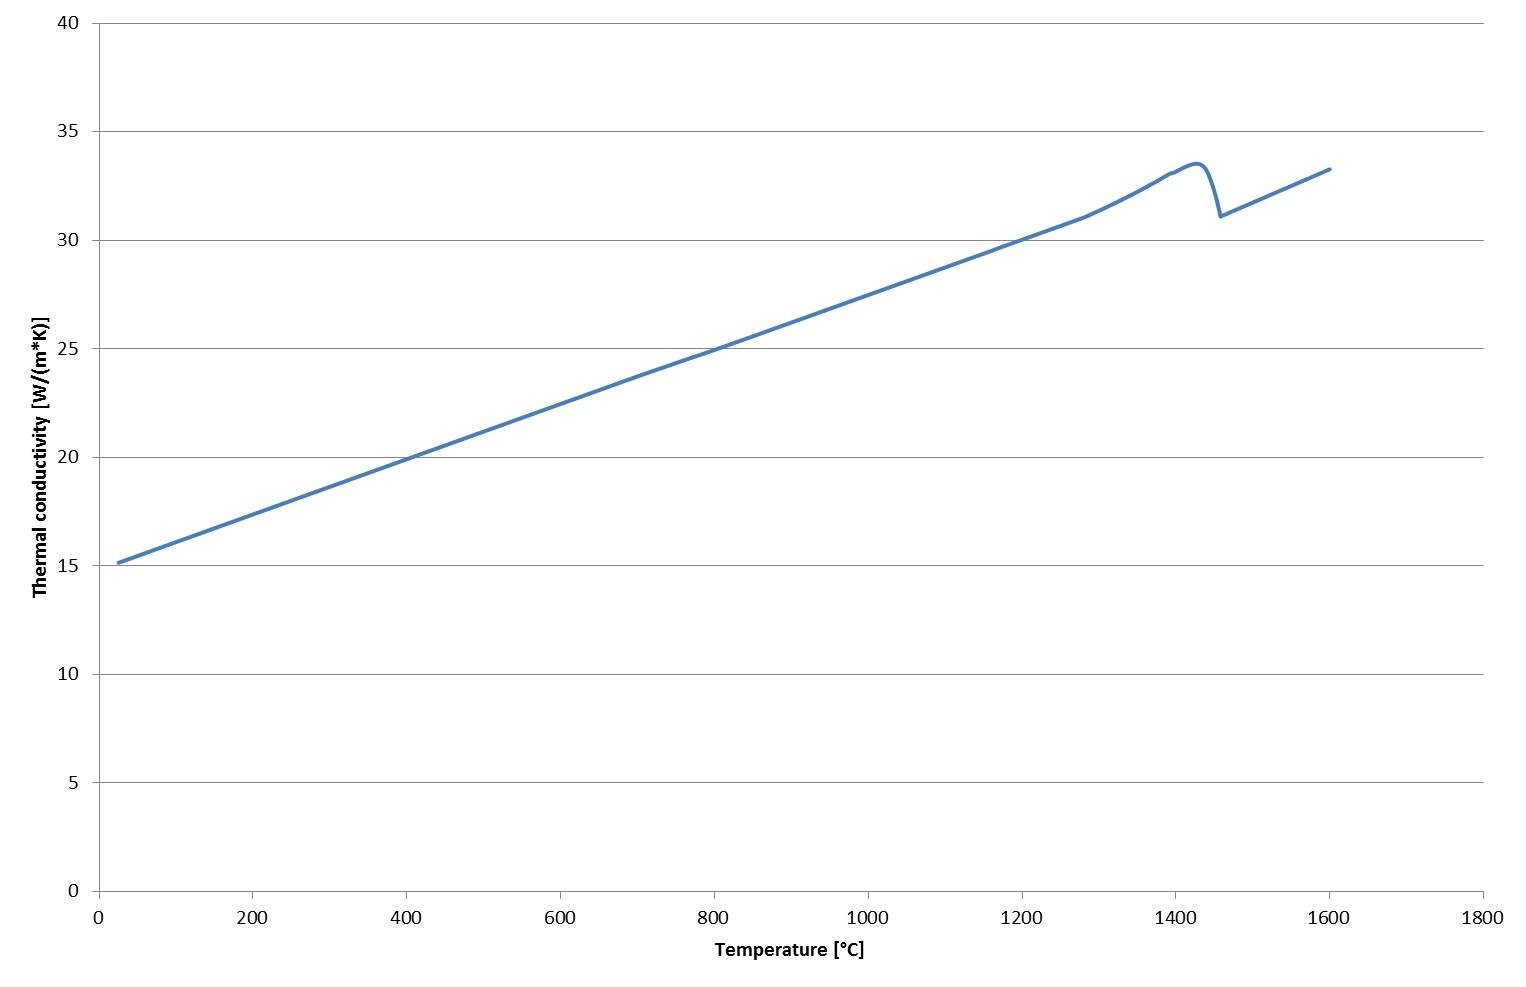
\includegraphics[width=0.8\textwidth]{images/thermalconductivity}
 \caption{Thermal conductivity of 1.4301}
 \label{img:thermalconductivity}
\end{figure}

\begin{figure}[htbp]
 \centering
 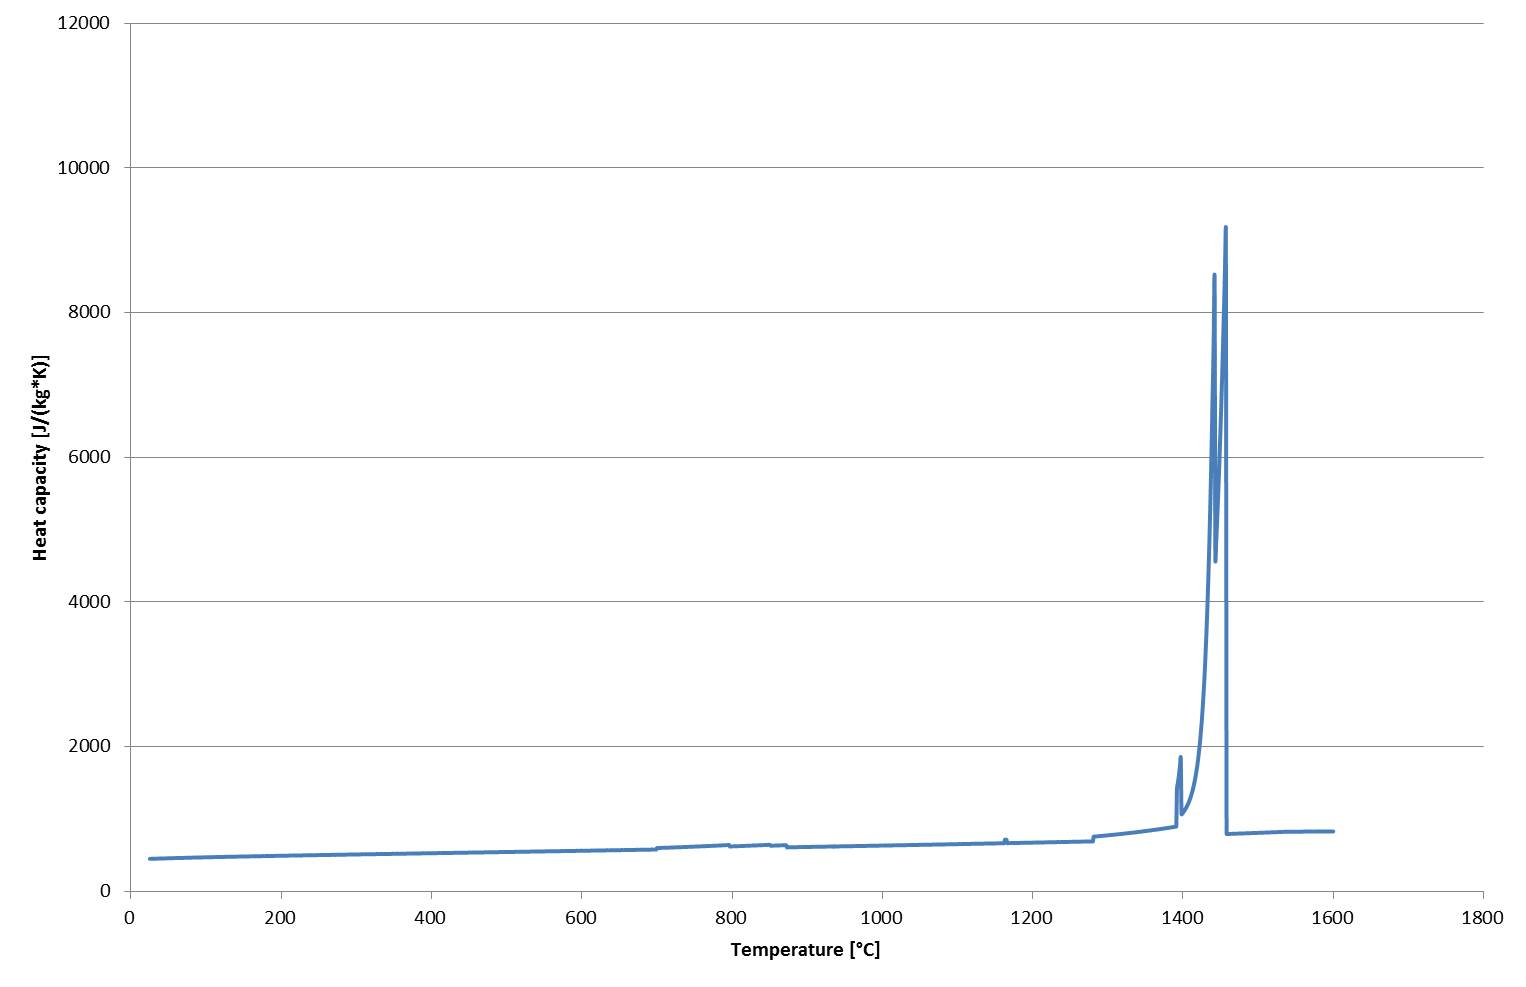
\includegraphics[width=0.8\textwidth]{images/heatcapacity}
 \caption{Heat capacity of 1.4301}
 \label{img:heatcapacity}
\end{figure}

\begin{figure}[htbp]
 \centering
 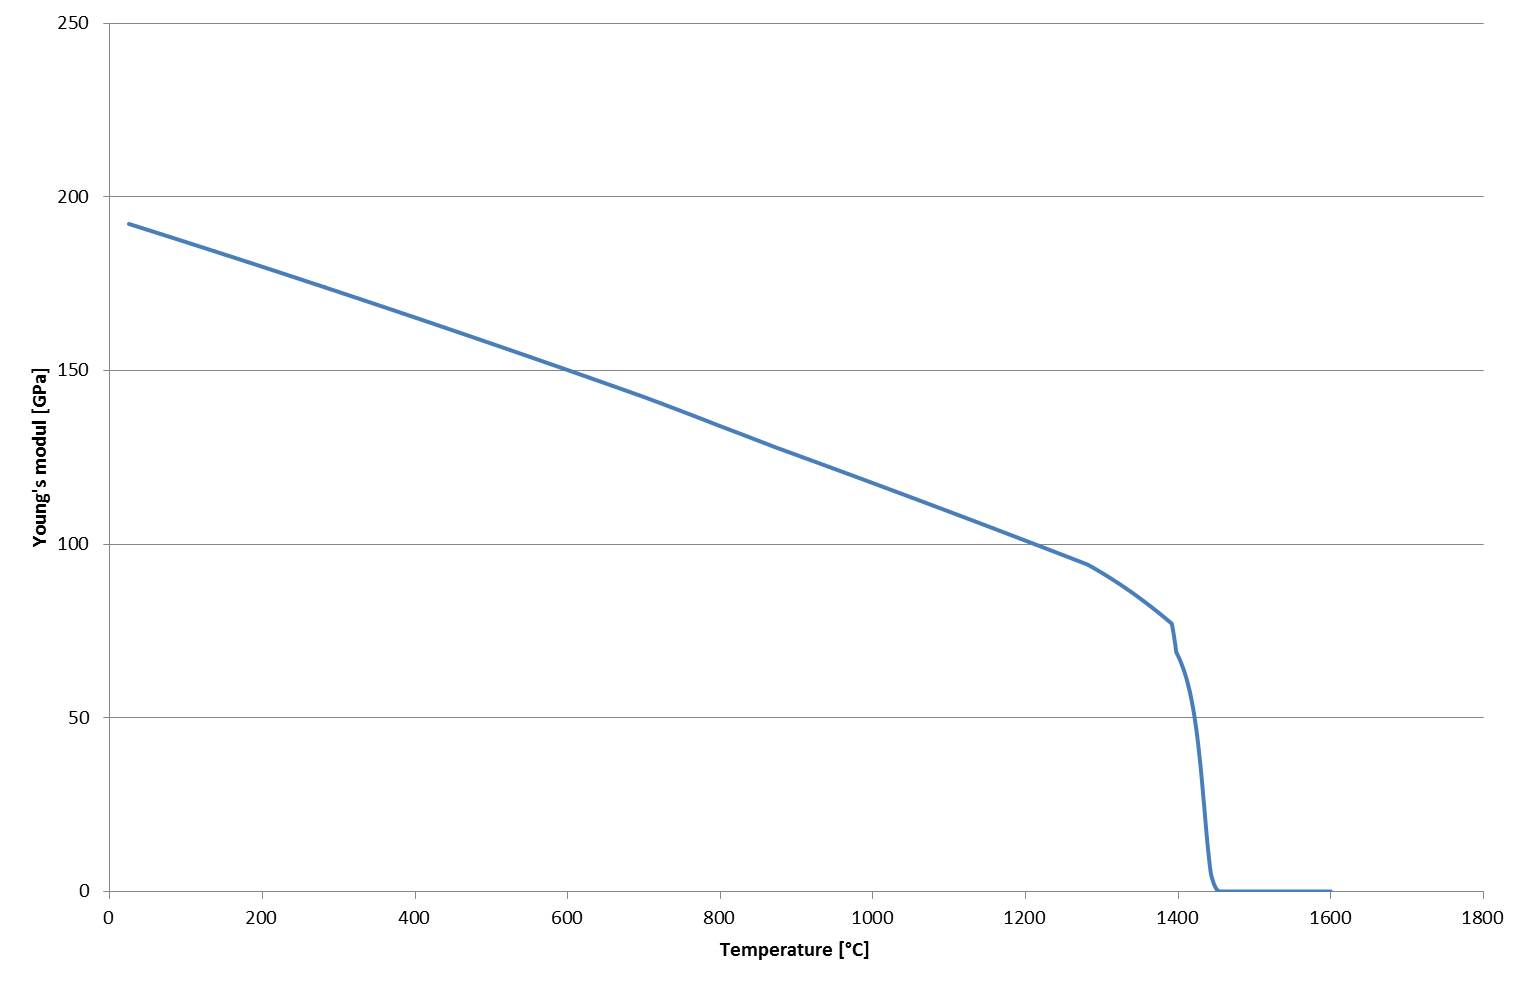
\includegraphics[width=0.8\textwidth]{images/youngsmodul}
 \caption{Young's modul of 1.4301}
 \label{img:youngsmodul}
\end{figure}

It is necessary that the data describes the whole temperature range of the process. Further parameters are set constant and are pictured in \ref{table:processparameter}. 

\begin{table}[htbp]%[width=0.8\textwidth]
 \centering
 \caption{Constant process parameters (reference temperature 20°C)}
 \begin{tabular}{|c|c|c|}
 \hline
 Poison&0,3&-\\
 \hline
 Thermal expansion&0,000012&[1/K]\\
 \hline
 Emissivity&0,7&-\\
 \hline
 Heat transfer coeff.&4,5&[W/(m²K)]\\
 \hline
 Friction coeff.&0,4&-\\
 \hline
 Dissipation&0,9&\%\\
 \hline
 \end{tabular}
 \label{table:processparameter}
\end{table}

\subsection{Forging plan (ForgeBase)}
The settings of the forging simulation are based on the calculation of the forging software ForgeBase \ref{table:forgingplan}. The simulations are done for a four passes process on a block (workpiece - WP) with the dimensions of 150mm in height as well as in width and 600mm in length. However, only 400mm of the length are forged. The rest is provided for the manipulator to hold and move the WP. The WP is set as a plastic solid and is meshed with a brick mesh with 12544 elements. The upper and lower dies are set as rigid object. The manipulator is set up as a spring with a stiffness of 175 N/mm and the maximum clamping force of 222,4 kN.\par 

The passes in the simulation vary in height reduction and bite ratio. Between the passes the WP is rotated in positive and negative direction with 90° rotation angle. There are two models of movement. On the one hand the bottom die is fixed, though the top die moves with a speed of 80mm/s (Simufact). On the other hand the top and the bottom die move with a speed of 40mm/s (DEFORM; PEP/LARSTRAN).

\begin{figure}[htbp]
 \centering
 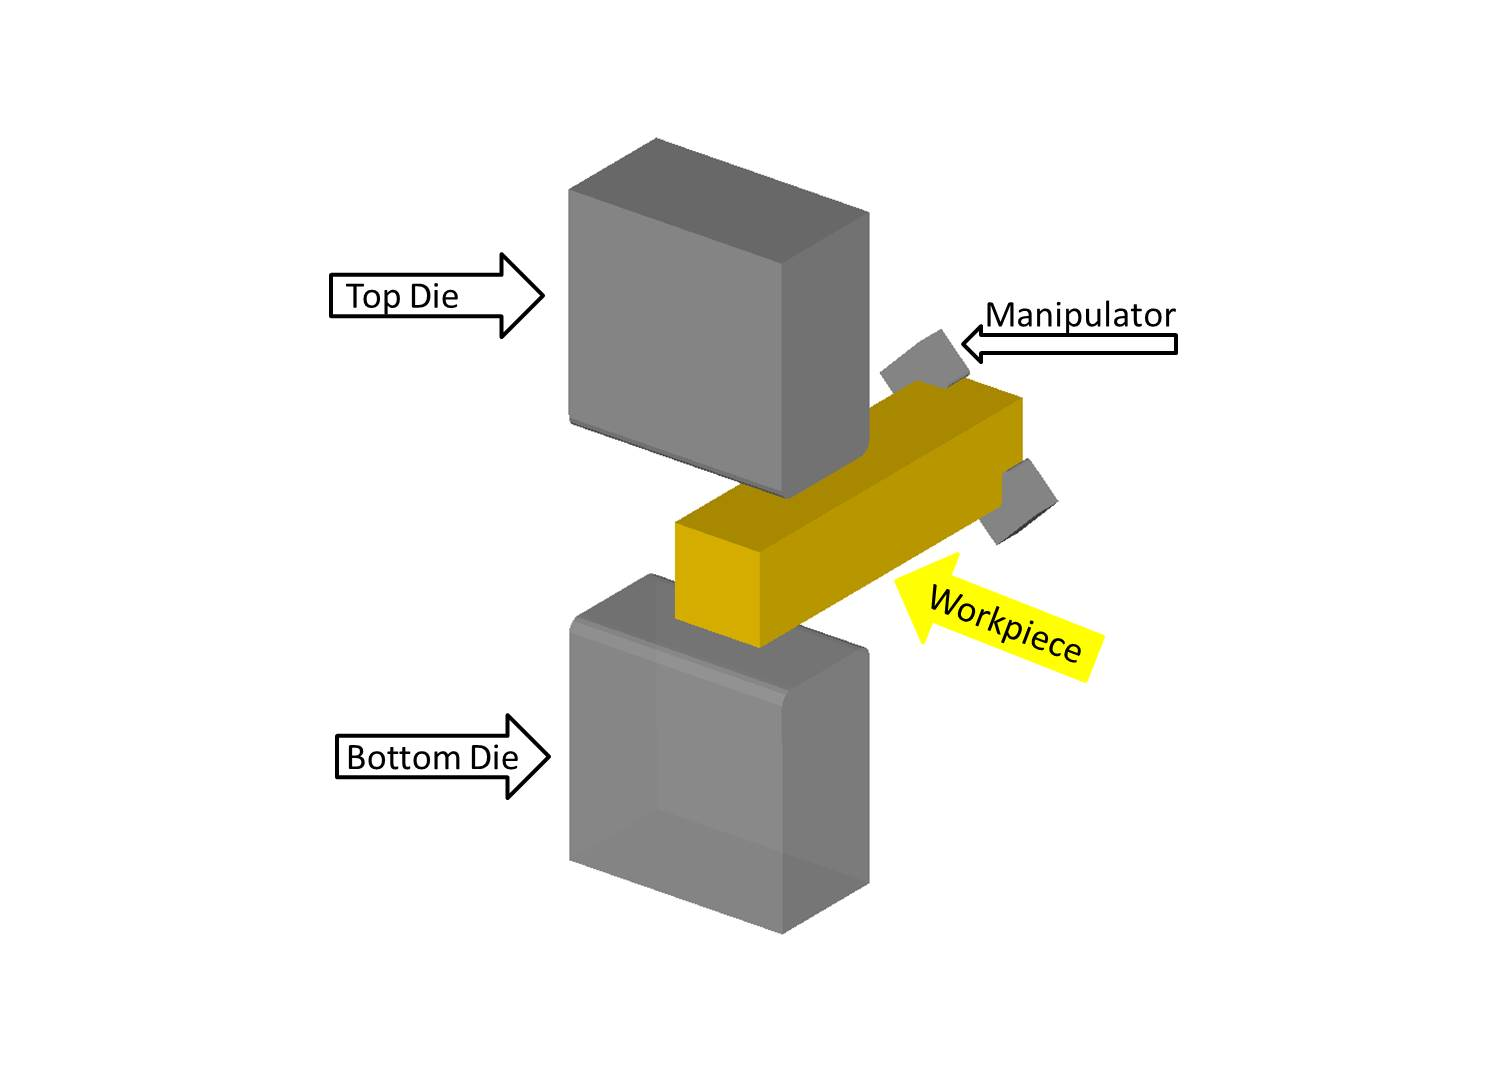
\includegraphics[width=0.8\textwidth]{images/processsetup}
 \caption{Illustration of the process setup from DEFORM}
 \label{img:processsetup}
\end{figure}

\begin{table}[htbp]%[width=1\textwidth]
 \footnotesize
 \centering
 \caption{Forging plan from ForgeBase}
 \begin{tabular}{|c|c|c|c|c|c|c|c|}
 \hline
 Pass Nr.&Reduction&Height 1&Width 1&Height 2&Width 2&Rotation&Bite width\\
 & [mm] & [mm] & [mm] & [mm] & [mm] & [$^{\circ}$] & [mm]\\
 \hline
 0&0&150&150&150&150&0&0\\
 \hline
 1&28&122&162&122&162&0&105\\
 \hline
 2&30&132&132&132&132&90&85\\
 \hline
 3&25&107&143&107&143&-90&92\\
 \hline
 4&27&116&116&116&116&90&75\\
 \hline
 \end{tabular}
 \label{table:forgingplan}
\end{table}

Moreover, the heat treatment before and during the process is of great importance. Before the first pass starts, the WP gets heated up to 1200°C for 2 hours. It is vital, that the WP does have a homogeneous distribution. During the forging passes, heat is getting lost by the effects of emission and the heat transfers to the dies. Because of that, a second heat is necessary between the second and the third pass. The WP is heated up again to 1200°C within 1 hour. After the last pass the WP cools down upon air to room temperature.

\section{Material modeling}
This chapter deals with the concept of material modeling based on semi-empirical equations. At first there will be a short overview of the mechanisms of recovery and recrystallization and after that a review of common models describing the evolution of microstructure during hot forming and a way to integrate them into common FEM-software.\par 

\subsection{Recovery and recrystallization}
The flow stress is highly dependent on microstructural softening and hardening mechanism during forming. In addition, these mechanisms are influenced by the temperature, strain rate and strain.\par 

During hot forming, defects are generated within the crystal lattice. According to Gottstein \cite{GOT07} the defects can be distinguished respecting their dimensions. Especially one dimensional defects called dislocations, are the carriers of plastic deformation and therefore crucial for hot working. During hot deformation the density of dislocations rises and hence the resistance of the material to deformation rises too. At a certain point the stored energy in the material is high enough to induce dynamic recovery (DRV) or dynamic recrystallization (DRX). These mechanisms cause softening of the material.\par 

DRV leads to equilibrium between hardening and softening. However DRX leads to a softened material. The effects of DRV and DRX can be well seen in the warm flow curve behavior, see \ref{img:warmflowcurves}.

\begin{figure}[htbp]
 \centering
 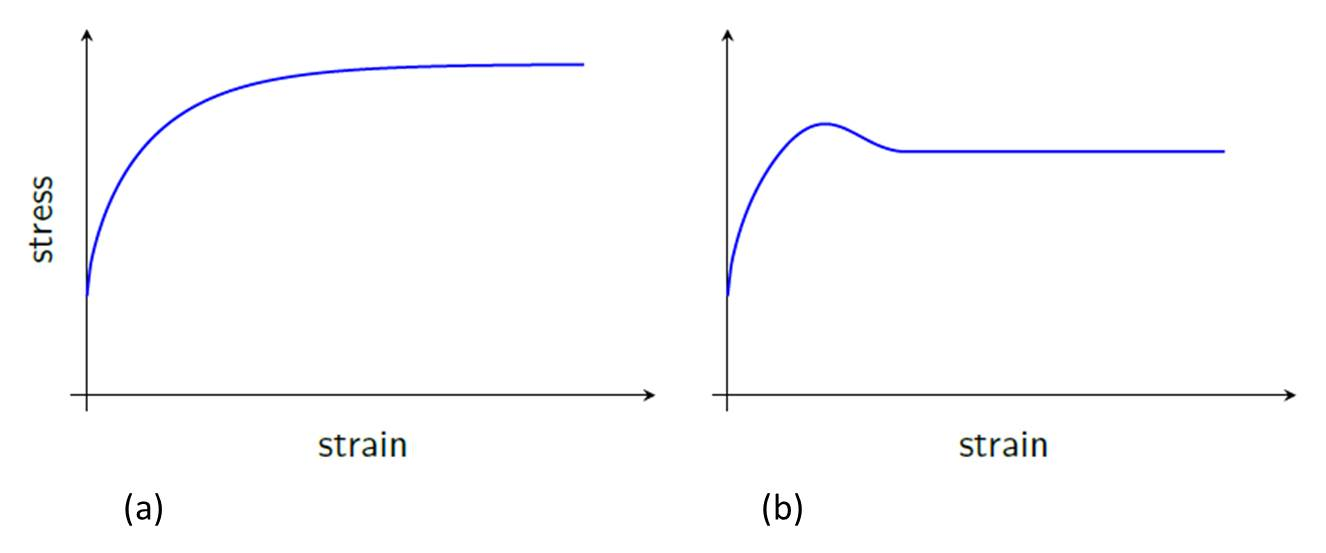
\includegraphics[width=0.8\textwidth]{images/warmflowcurves}
 \caption{Warm flow curves when recovery (a) or recrystallization (b) is predominant \cite{LOH10}}
 \label{img:warmflowcurves}
\end{figure}

The softening effect of DRV and therefore the reduced level of stress with increasing strain is based on the rearrangement and annihilation of dislocations [Gottstein]. During DRX new grains are built and grow at spots with low specific energy. Both effects lead to a totally refined microstructure.\par

After hot forming, remaining dislocations can still store a great amount of energy. This energy can be enough to cause static recovery (SRV) or static recrystallization (SRX). These processes take place during heat treatment after warm forming. The softening effects are the same as in DRV or DRX. The driving force drops during SRV and SRX and only when there is enough energy stored, SRV and SRX lead to a fully refined microstructure.\par 

After or parallel to SRV and SRX, grain growth (GG) can take place. The driving force is the reduction of stored energy. During grain growth the nucleated grains grow by using up the old grain structure.\par 

\ref{img:recovandrecrystwarmforming} gives a short summary about the recovery, recrystallization and grain growth mechanisms during warm forming.

\begin{figure}[htbp]
 \centering
 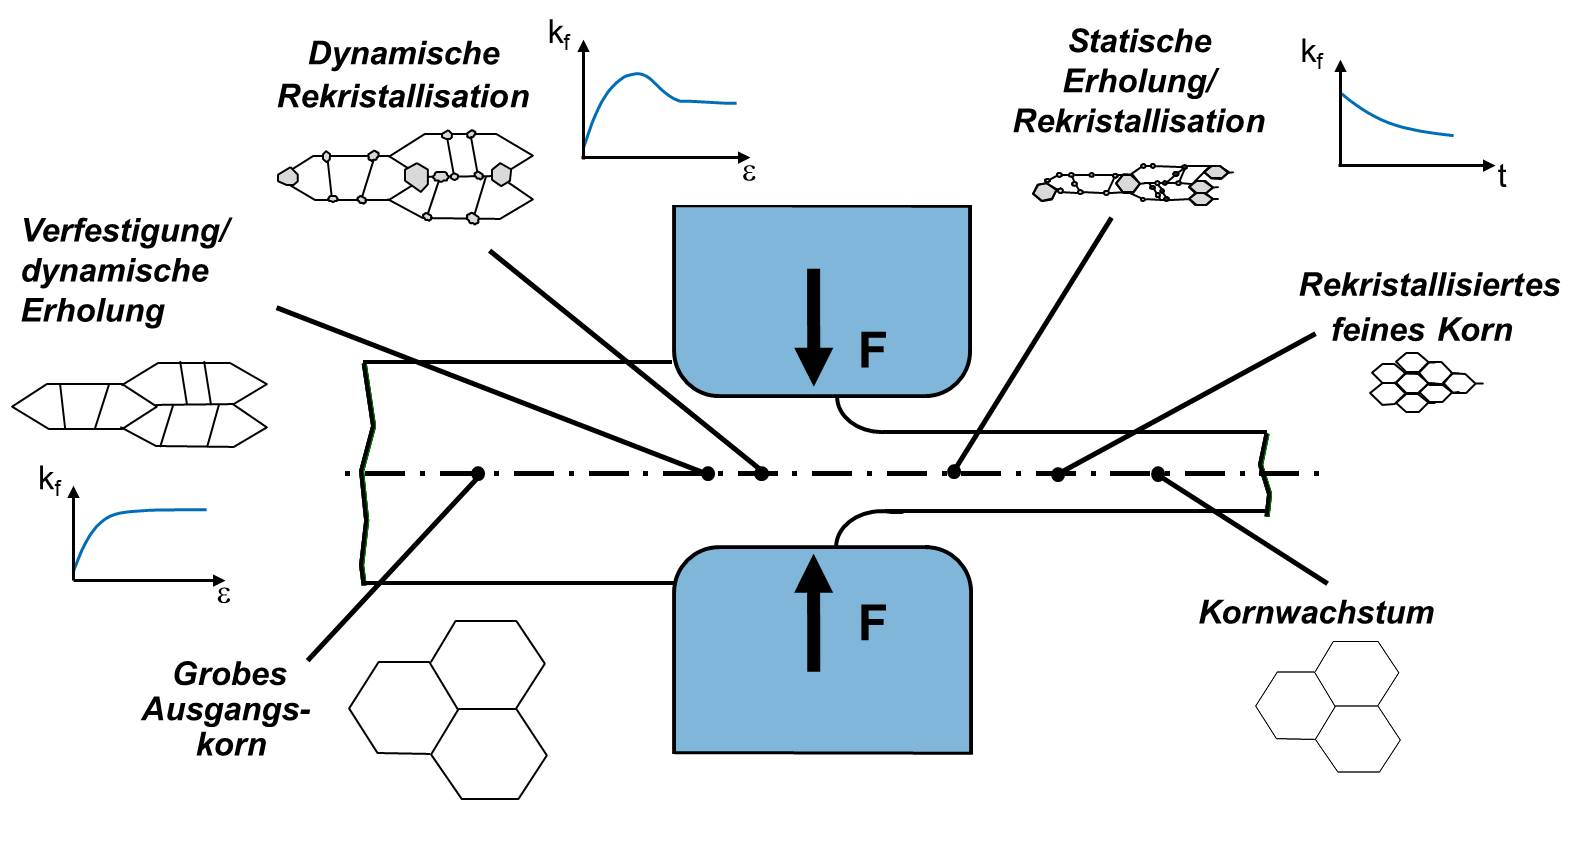
\includegraphics[width=0.8\textwidth]{images/recovandrecrystwarmforming}
 \caption{Recovery and recrystallization mechanisms during warm forming}
 \label{img:recovandrecrystwarmforming}
\end{figure}

The flow curves \ref{img:flowcurves} are essential for the determination of the recrystallization kinetics and the fraction of recrystallized material. Therefore it is the basis for the creation of a microstructure model. At the IBF, flow curves are determined by isothermal compression tests at cylindrical specimens with an eight to diameter ratio of 1,5. For the 1.4301 tests have been carried out at temperatures ranging from $900 - 1250 ^{\circ}C$ and strain rates of $0,05 - 100 s^{-1}$ \ref{img:flowcurves}.

\begin{figure}[htbp]
 \centering
 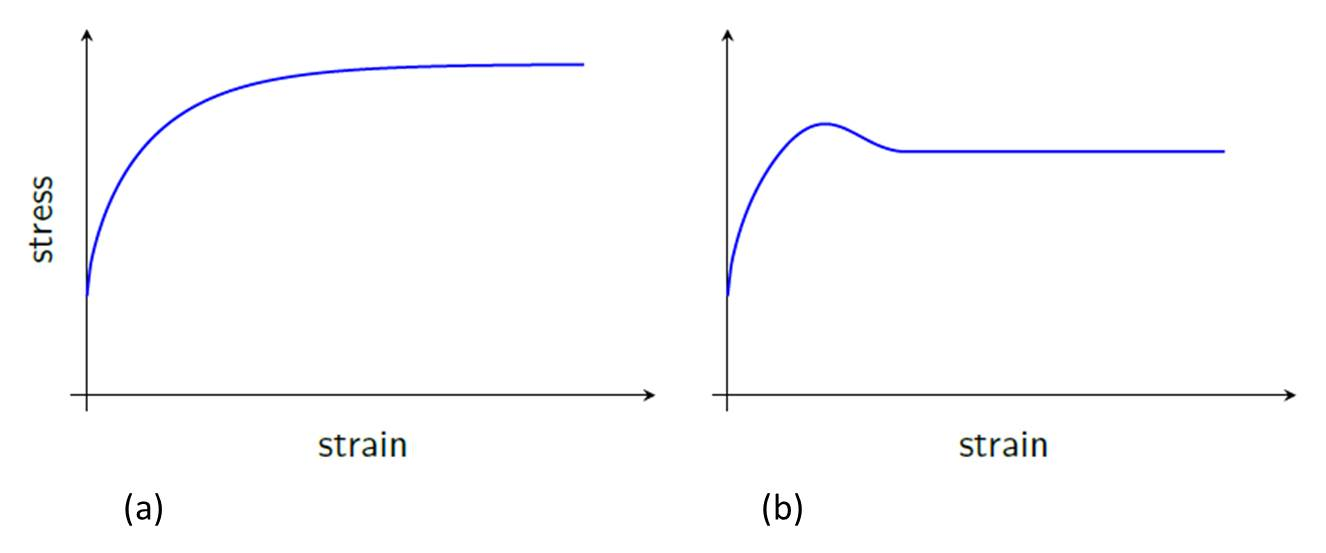
\includegraphics[width=0.8\textwidth]{images/flowcurves}
 \caption{Determined flow curves of 1.4301 (temperature range: 900-1250°C)}
 \label{img:flowcurves}
\end{figure}

For the semi empirical material model given by Deghan Manshadi \cite{DEG08} the special strain values are of great importance. These strain states are seen in \ref{img:stressstrainpoints}. There is the peak strain $\varepsilon_{p}$, the strain of steady state $\varepsilon_{ss}$, and not seen in \ref{img:stressstrainpoints} the critical strain $\varepsilon_{c}$ which is located at 60\%\ of the peak strain. The stresses at these characteristic points are also of importance.

\begin{figure}[htbp]
 \centering
 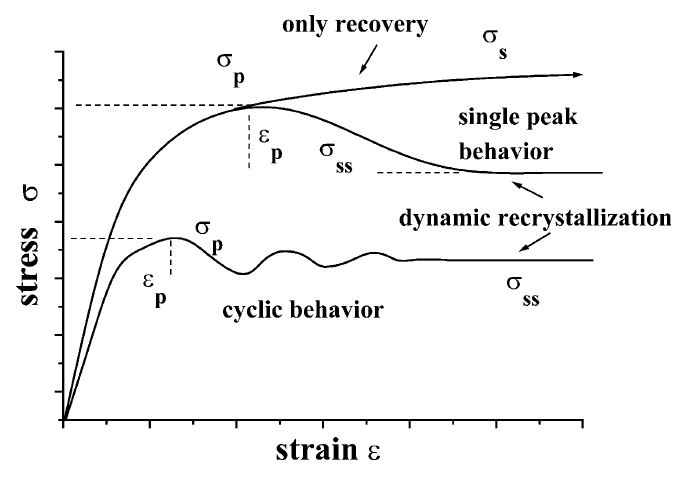
\includegraphics[width=0.8\textwidth]{images/stressstrainpoints}
 \caption{Warm flow curves with characteristic stress and strain points \cite{ELW03}}
 \label{img:stressstrainpoints}
\end{figure}

They can also be calculated by:
\begin{equation}
 \varepsilon_{p} = 3,6\cdot10^{-3}d_{0}^{0}\cdot Z^{0,15}
\end{equation}

\begin{equation}
 \varepsilon_{c} = 0,6\cdot\varepsilon_{p}
\end{equation}

\begin{equation}
 \varepsilon_{ss} = 0,00598\cdot d_{0}^{0}\cdot Z^{0,1536}
\end{equation}

\subsection{Semi emprirical material models}
For the prediction of microstructural evolution semi-empirical models are used for many years. Lohmar and Karhausen gave a detailed overlook over the common models used in warm forming \cite{LOH10}\cite{KAR94}.\par 

The JMAK-equation is a way to calculate the fraction of recrystallization X \ref{img:JMAK} for the different recrystallization mechanisms DRX and SRX. In this work the equation for the calculation of DRX and SRX published by Dehgan Manshadi is used \cite{DEH08}.

\begin{equation}
 X = 1 - exp\left( log\left( 1-0,95\right) \cdot\left( \frac{\varepsilon_{eff}-\varepsilon_{c}}{\varepsilon_{x}}\right) ^{1,3}\right)
\end{equation}

\begin{equation}
 X = 1 - exp\left( log\left( 1-0,5\right) \cdot\left( \frac{t_{SRX}}{t_{50}}\right) ^{1,1}\right)
\end{equation}

Where $t_{50}$ is the time where 50\% recrystallization took place \ref{img:JMAK}:

\begin{equation}
 t_{50} = 8\cdot10^{-9}\varepsilon^{-1,5}\cdot Z^{-0,42}exp\left( \frac{375000}{R\cdot T}\right)
\end{equation}

\begin{figure}[htbp]
 \centering
 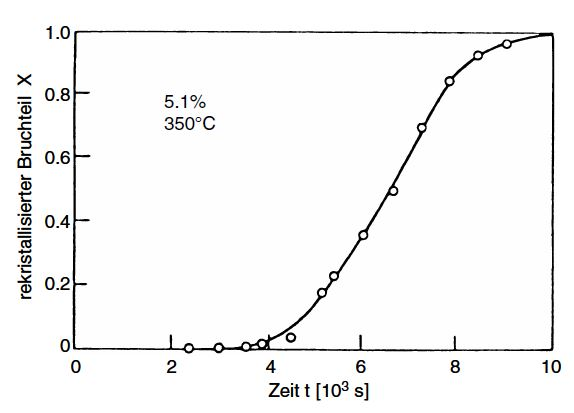
\includegraphics[width=0.8\textwidth]{images/JMAK}
 \caption{Fraction of recrysrallization X}
 \label{img:JMAK}
\end{figure}

A lot of these models relate the stress behavior to the strain rate $\dot{\varepsilon}$ and the Temperature T. A popular way to describe this is given by the Zener-Hollomon parameter Z \cite{ZEN44}:

\begin{equation}
 Z =  \varepsilon\cdot exp\left( \frac{Q}{R\cdot T}\right)
\end{equation}

These equations lead to the determination of the grain size $d_{DRX}$ and $d_{SRX}$ \cite{DEH08}:

\begin{equation}
 d_{DRX} =  5916\cdot Z^{-0,1748}
\end{equation}

\begin{equation}
 d_{SRX} =  4,7\cdot10^{2}\cdot\varphi_{SRX^{-1}}\cdot100^{0,3}\cdot Z^{-0,1}
\end{equation}

\section{Validation}

For the modelling of the described process, different software packages are available. Specifically, DEFORM-3D from Scientific Forming Technologies Corporation,Columbus, USA, FORGE from Transvalor, Mougins, France, and a combination of PEP (Pre- and Postprocessing Environment for Programmers) developed at IBF and LARSTRAN from LASSO Ingenieurgesellschaft mbH, Leinfelden, Germany have been used. These packages differ in their ease of use and freedom in modelling. A comparison of both usability and results will be made here.

\subsection{DEFORM-3D}

\subsection{FORGE}

\subsection{PEP/LARSTRAN}

\include{microstructure_results}
\section{Summary}

\section{Outlook}

The results of microstucture modelling have shown that small strain rates result in large values for the dynamically recrystallized volume fraction. This effect is due to the limitations of using absolute thresholds for microstructural parameters. The models should be extended to give a more dynamic model which allows a bigger range of these paramenters.

Furthermore, a systematic approach to the comparison of various FEM packages with each other and with reality should involve, as a first step, the research of the capabilities of the involved packages and the development of an according model process. Also, an even more detailed process model should be set up, using the same time increments, mesh, boundary conditions etc.

Lastly, a validation of the results in a real process is necessary. This includes a validation of both the microstructural model with grain sizes measured during the process and the process parameters such as die forces and material temperature development.

\newpage
\listoffigures
\newpage
\bibliographystyle{alphadin}
\bibliography{hauptseminar_hibbe_nick_2014}
\include{appendix}
\end{document}
